%% LyX 2.2.2 created this file.  For more info, see http://www.lyx.org/.
%% Do not edit unless you really know what you are doing.
\documentclass[english]{beamer}
\usepackage{mathptmx}
\usepackage[latin9]{inputenc}
\usepackage{amsmath}
\usepackage{amssymb}
\usepackage{graphicx}
\usepackage[european]{circuitikz}
\ctikzset{tripoles/mos style/arrows}

\makeatletter

%%%%%%%%%%%%%%%%%%%%%%%%%%%%%% LyX specific LaTeX commands.
%% Because html converters don't know tabularnewline
\providecommand{\tabularnewline}{\\}

%%%%%%%%%%%%%%%%%%%%%%%%%%%%%% Textclass specific LaTeX commands.
 % this default might be overridden by plain title style
 \newcommand\makebeamertitle{\frame{\maketitle}}%
 % (ERT) argument for the TOC
 \AtBeginDocument{%
   \let\origtableofcontents=\tableofcontents
   \def\tableofcontents{\@ifnextchar[{\origtableofcontents}{\gobbletableofcontents}}
   \def\gobbletableofcontents#1{\origtableofcontents}
 }

%%%%%%%%%%%%%%%%%%%%%%%%%%%%%% User specified LaTeX commands.
\usetheme{Warsaw}
% or ...

\setbeamercovered{transparent}
% or whatever (possibly just delete it)

\makeatother

\usepackage{babel}
\begin{document}

\title[Designing a SCaM]{Analog Design for a Single-Chip atto Mote (SCaM) Microcontroller
}

\author[Kevavi]{Kevin Chen, Avi Pandey, Kevin Zheng}

\institute{University of California, Berkeley}

\date{Presentation 1}

\makebeamertitle

%\pgfdeclareimage[height=0.5cm]{institution-logo}{logo.png}
%\logo{\pgfuseimage{institution-logo}}

\AtBeginSubsection[]{%
  \frame<beamer>{ 
    \frametitle{Outline}   
    \tableofcontents[currentsection,currentsubsection] 
  }
}

%\beamerdefaultoverlayspecification{<+->}
\begin{frame}{Outline}

\tableofcontents{}
\end{frame}

\section{Preliminaries}

\subsection{Introductions}
\begin{frame}{Kevin Chen}
\begin{itemize}
\item Board Game Fanatic
\item Teaching EE16B
\item Perpetually trying to bring people to bowling or rock climbing
\item Fond of learning mostly-useless skills, like lock-picking
\end{itemize}
\end{frame}
%
\begin{frame}{Avi Pandey }
\begin{itemize}
\item Teaching EE16A
\item Tennis Enthusiast
\item Have taken apart and put back together an engine before (and gotten it to work)
\item Learned useless skills from Kevin (Like using a butterfly knife)
\end{itemize}
\end{frame}
%
\begin{frame}{Kevin Zheng}
\begin{itemize}
\item Open-source developer and FreeBSD contributor
\item Teaching EE 198: Hands-On Practical Electronics
\item Amateur radio operator
\item Tanguero
\end{itemize}
\end{frame}

\subsection{Block Diagram}
\begin{frame}{Block Diagram}

\begin{figure}

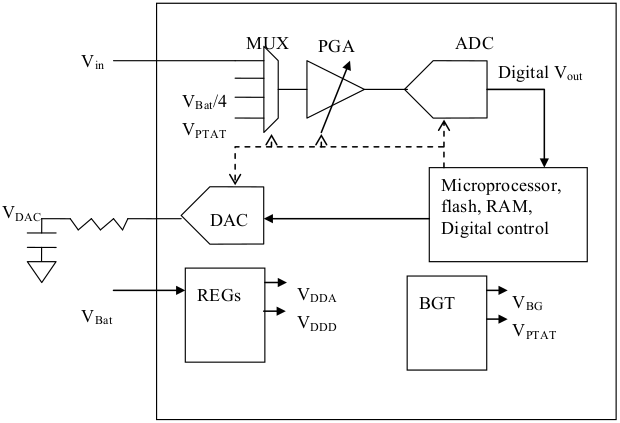
\includegraphics[width=0.7\linewidth]{block-diagram}

\end{figure}

\end{frame}

\section{Project Plans}

\subsection{Block Specifications}
\begin{frame}{Band Gap \& Temperature Sensor}
\begin{block}{Basic Specs}
\begin{itemize}
\item 1.2 V $\pm$ 5 mV across 0-70 $^\circ$C
\item PTAT voltage output
\end{itemize}
\end{block}
%
\begin{block}{Topology}
\begin{itemize}
\item Razavi band gap reference with extra branch for PTAT voltage generation
\item NMOS input op-amp
\end{itemize}
\end{block}
\end{frame}
%
\begin{frame}{Digital Regulator}
\begin{block}{Basic Specs}
\begin{itemize}
\item 1.2 V $\pm$ 120 mV across 0-70 $^\circ$C at 5 mA
\item Less than 400 mV dropout
\end{itemize}
\end{block}
%
\begin{block}{Topology}
\begin{itemize}
\item NMOS input componensated two-stage
\end{itemize}
\end{block}
\end{frame}
%
\begin{frame}{Analog Regulator}
\begin{block}{Basic Specs}
\begin{itemize}
\item 1.2 V $\pm$ 0.1 mV across 0-70 $^\circ$C at 5 mA
\item Less than 400 mV dropout
\end{itemize}
\end{block}
%
\begin{block}{Topology}
\begin{itemize}
\item NMOS input componensated two-stage
\end{itemize}
\end{block}
\end{frame}
%
\begin{frame}{ADC}
\begin{block}{Basic Specs}
\begin{itemize}
\item 8-bit SAR
\item 100k samples/s $\implies 10\mu s$/sample 
\item Input range 0-1 V
\end{itemize}
\end{block}
%
\begin{block}{Topology}
\begin{itemize}
\item Strongarm latch comparing at $\text{V}_\text{REF}$
\end{itemize}
\end{block}
\end{frame}
%
\begin{frame}{Multiplexer}
\begin{block}{Basic Specs}
\begin{itemize}
\item 0-1 V analog input voltage range
\item 4 to 1 MUX.
\item 10 $\tau$ RC delay less than 1$\mu$s. 
\end{itemize}
\end{block}
%
\begin{block}{Topology}
\begin{itemize}
\item Built out of two 2 to 1 MUXs.
\item Transmission Gate topology. 
\end{itemize}
\end{block}
\end{frame}
%
\begin{frame}{PGA}
\begin{block}{Basic Specs}
\begin{itemize}
\item Programmable gain between 1-8
\item Less than 0.4\% gain error 
\item Drives 1024 fF ADC
\item Common mode input range 0-1 V
\end{itemize}
\end{block}
%
\begin{block}{Topology}
\begin{itemize}
\item PMOS input folded cascode 2 stage
\begin{itemize}
\item Input with 0 V CM
\item Output with 0 V - 1 V swing
\item Settles to 0.4\% in 4 $\mu$s
\item Unity gain stable with load capacitance from 4fF to 1024fF
\end{itemize}
\end{itemize}
\end{block}
\end{frame}
%


\subsection{Preliminary Results}
\begin{frame}{Band Gap}
\begin{itemize}
\item We had zero temperature coefficient at 25 $^\circ$C
\item Less than 20 mV variation across -40 $^\circ$C to 85 $^\circ$C
\end{itemize}
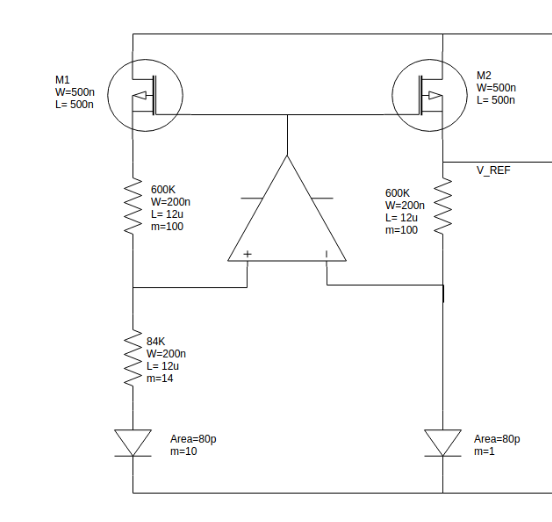
\includegraphics[scale=0.3]{band_gap_circuit.png}
\end{frame}
%
\begin{frame}{Folded Cascode w/PMOS input}
\begin{itemize}
\item 0-0.9 V common-mode input range
\item Better than 2250x gain from -40 $^\circ$C to 85 $^\circ$C
\item Less than 0.4\% gain error
\item Some bias issues
\end{itemize}
 \begin{circuitikz}[scale = 0.5, transform shape]
        \draw
        (2,5) node[pmos](m6) {} 
        node [anchor=west]{$\frac{4\mu m}{1\mu m}$}
        (1,3) node[pmos](m1a) {}
        node [anchor=west]{$\frac{2\mu m}{1\mu m}$}
        (3,3) node[pmos, xscale=-1](m1b) {}
        (m6.D) -| (m1a.S)
        (m6.D) -| (m1b.S)

        (m1a.D) to[short] ++(0,-2)
        (m1b.D) to[short] ++(0,-2)

        (5,5) node[pmos, xscale=-1](m4a) {}
        (8,5) node[pmos](m4b) {}
        node [anchor=west]{$\frac{2\mu m}{1\mu m}$}
        (5,3) node[pmos, xscale=-1](m3a) {}
        (8,3) node[pmos](m3b) {}
        node [anchor=west]{$\frac{2\mu m}{1\mu m}$}
        
        (m4a.G) -- (m4b.G)
        (m3a.G) -- (m3b.G)
        (m4a.D) -- (m3a.S)
        (m4b.D) -- (m3b.S)
        (m4a.G) |- (m3a.D)
        (m3a.G) to[short] ++(0.5,0)
        node[anchor=north]{$V_{B4}$}
        
        (5,1) node[nmos, xscale=-1](m2a){}
        (8,1) node[nmos](m2b){}
        node [anchor=west]{$\frac{1\mu m}{1\mu m}$}
        (5,-1) node[nmos, xscale=-1](m5a){}
        (8,-1) node[nmos](m5b){}
        node [anchor=west]{$\frac{2\mu m}{1\mu m}$}

        (m5a.G) -- (m5b.G)
        (m2a.G) -- (m2b.G)
        (m2a.S) -- (m5a.D)
        (m2b.S) -- (m5b.D)

        (m2a.D) -- (m3a.D)
        (m2b.D) -- (m3b.D)
        (m1b.D) to[short] ++(0,-2)
        -| (m5b.D)
        (m1a.D) to[short] ++(0,-2.5) 
        -| (m5a.D)
        (m6.S) -- (m4a.S)
        (m6.S) -- (m4b.S)
        (m6.S) to[short] ++(-0.5,0)
        (m4b.S) to[short] ++(0.5,0)
        
        (m5a.S) -- (m5b.S)
        (m5a.S) to[short] ++(-3.5,0)
        (m5b.S) to[short] ++(0.5,0)
        
        (m1a.G) node[anchor=east]{$V_-$}
        (m1b.G) node[anchor=west]{$V_+$}
        
        (m6.G) node[anchor=east]{$V_{B1}$}
        (m5a.G) to[short] ++(0.5,0)
        node[anchor=south]{$V_{B2}$}
        (m2a.G) to[short] ++(0.5,0)
        node[anchor=south]{$V_{B3}$}
        (m4a.S) node[anchor=south]{$V_\text{DD}$}
        (m5a.S) node[anchor=north]{GND}

        (11,-1) node[nmos](nmosa){}
        node[anchor=west]{$\frac{1\mu m}{1\mu m}$} 
        (11,5) node[pmos](pmosa){}
        node[anchor=west]{$\frac{1\mu m}{1\mu m}$}
        (nmosa.D) -- (pmosa.D)
        (nmosa.S) -- (m5a.S)
        (pmosa.S) -- (m4b.S)
        (nmosa.G) node[anchor=east]{$V_{B2}$}
        (pmosa.G) |- (8,2)
        ;
    \end{circuitikz}

\end{frame}

\subsection{Responsibilities}
\begin{frame}{Responsibilities}

\begin{tabular}{|c|c|c|c|}
\hline 
 & ADC & PGA/MUX & BG/REG\tabularnewline
\hline 
\hline 
Topology & Pandey & Chen & Zheng\tabularnewline
\hline 
Amplifier & Zheng & Pandey & Chen\tabularnewline
\hline 
Verification & Chen & Zheng & Pandey\tabularnewline
\hline 
\end{tabular}
\end{frame}
%
\begin{frame}{Milestones}
\begin{itemize}
\item Blocks complete and implemented with ideal amplifiers (4/20)
\item System-level testbenches complete; first integration (4/21)
\item Ideal amplifiers replaced with real amplifiers (4/25)
\item Sanity check and verification (4/26)
\item Extras, final integration and submission (4/28)
\end{itemize}
\end{frame}
%
\begin{frame}{Scoring}
\begin{itemize}
\item 5\%: Meeting internal milestone dates
\item 55\%: Functional SCaM units meeting specs
\item 40\%: Functional SCaM system. 
\end{itemize}
\end{frame}

\end{document}
